\section{Aufgabenliste}
\label{sec:PlanungAufgabenliste}

\begin{enumerate}

\item \textbf{\emph{Planung:}}
\begin{itemize}
\item Aufgabenliste erstellen
\item Zeiteinteilung
\item Meilensteine definieren
\item Gantt erstellen
\end{itemize}

\item \textbf{\emph{Analyse:}}
\begin{itemize}
\item Recherche CNN
\item Recherche Testdaten
\item Recherche C++ Details
\item Anforderungen definieren
\item Use Cases
\item weitere Analysen
\item Schreiben Analyse
\end{itemize}

\item \textbf{\emph{Design:}}
\begin{itemize}
\item GUI konzipieren
\item Wireframes zeichnen
\item Konsolenbefehle definieren
\item Konsolen Output definieren
\end{itemize}

\item \textbf{\emph{Realisation:}}
\begin{itemize}
\item Input Layer realisieren
\item Convolutional Layer realisieren
\item Pooling Layer realisieren
\item Dense Layer Klasse schreiben
\item Output Layer erstellen
\item CNN-Model erstellen
\item CNN-Model trainieren
\item GUI auf CNN-Model setzen
\item GPU-Anbindung implementieren
\item Kommentare schreiben
\item weitere Verbesserungen vornehmen
\item Bufferzeit programmieren
\end{itemize}

\item \textbf{\emph{Dokumentieren:}}
\begin{itemize}
\item Schreiben
\end{itemize}

\item \textbf{\emph{Testen:}}
\begin{itemize}
\item Testliste kreieren
\item Tests implementieren
\item Tests durchf�hren
\end{itemize}

\item \textbf{\emph{Deployment:}}
\begin{itemize}
\item Projekt als EXE bauen
\item Build Anleitung kreieren
\end{itemize}

\item \textbf{\emph{Pr�sentation:}}
\begin{itemize}
\item Pr�sentation erstellen
\end{itemize}

\item \textbf{\emph{Buffer allgemein}}
\end{enumerate}

\section{Meilensteine}
\label{sec:PlanungMeilensteine}

\begin{xltabular}{\linewidth}{|X|X|}
\hline
Meilenstein-Name & Datum
\\\hline
Vorbereitungen abgeschlossen & 20.10.2023
\\\hline
CNN-Model Kreation abgeschlossen & 10.11.2023
\\\hline
Dokumentation abgeschlossen & 01.12.2023
\\\hline
Produkt abgeschlossen & 05.01.2024
\\\hline
Projekt abgeschlossen & 10.02.2024
\\\hline
\hl{Projekt abgegeben} & \hl{23.02.2024}
\\\hline
\end{xltabular}

\section{Gantt}
\label{sec:PlanungGantt}
\begin{landscape}

\begin{figure}[tb]
	\centering
		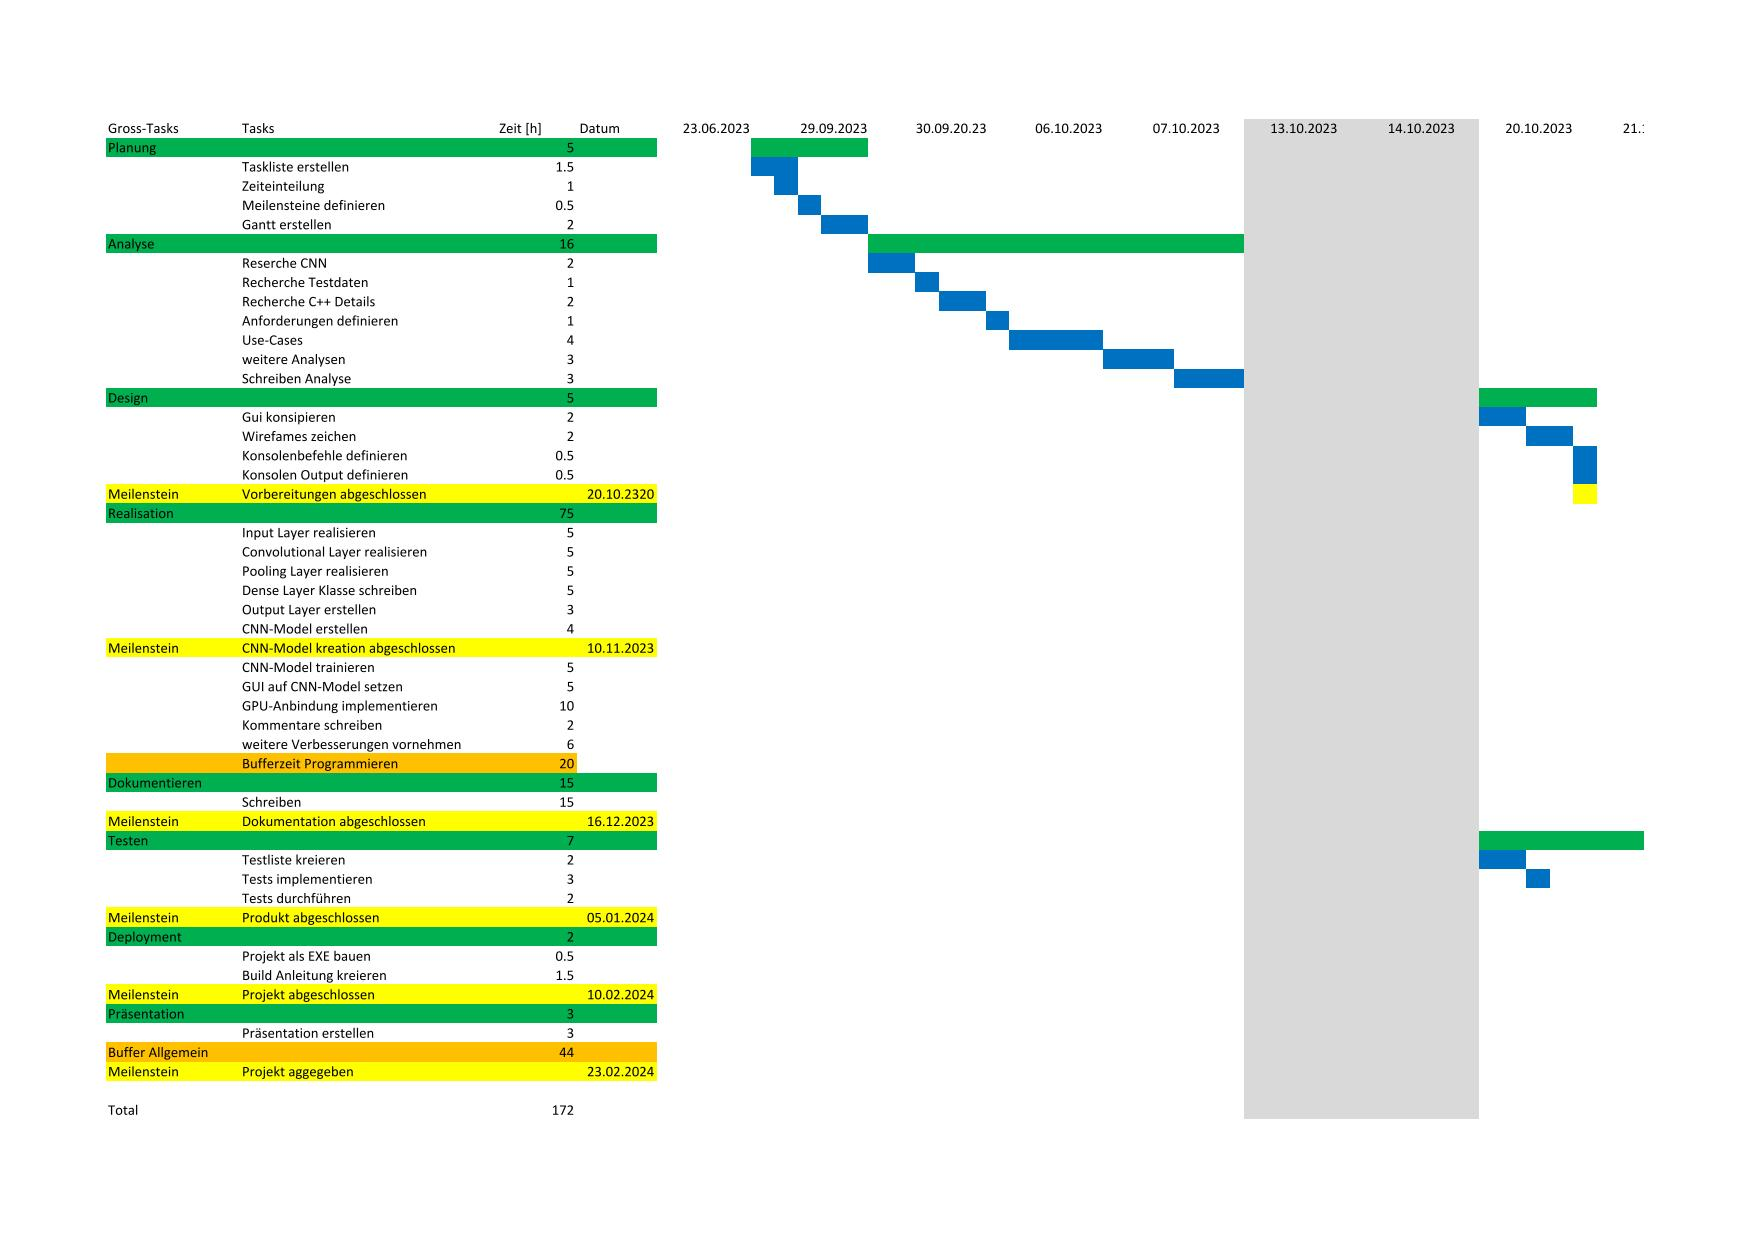
\includegraphics[width=\pdfpagewidth]{images/gantt1.jpg}
	\label{fig:planunggantt1}
\end{figure}

\begin{figure}[tb]
	\centering
		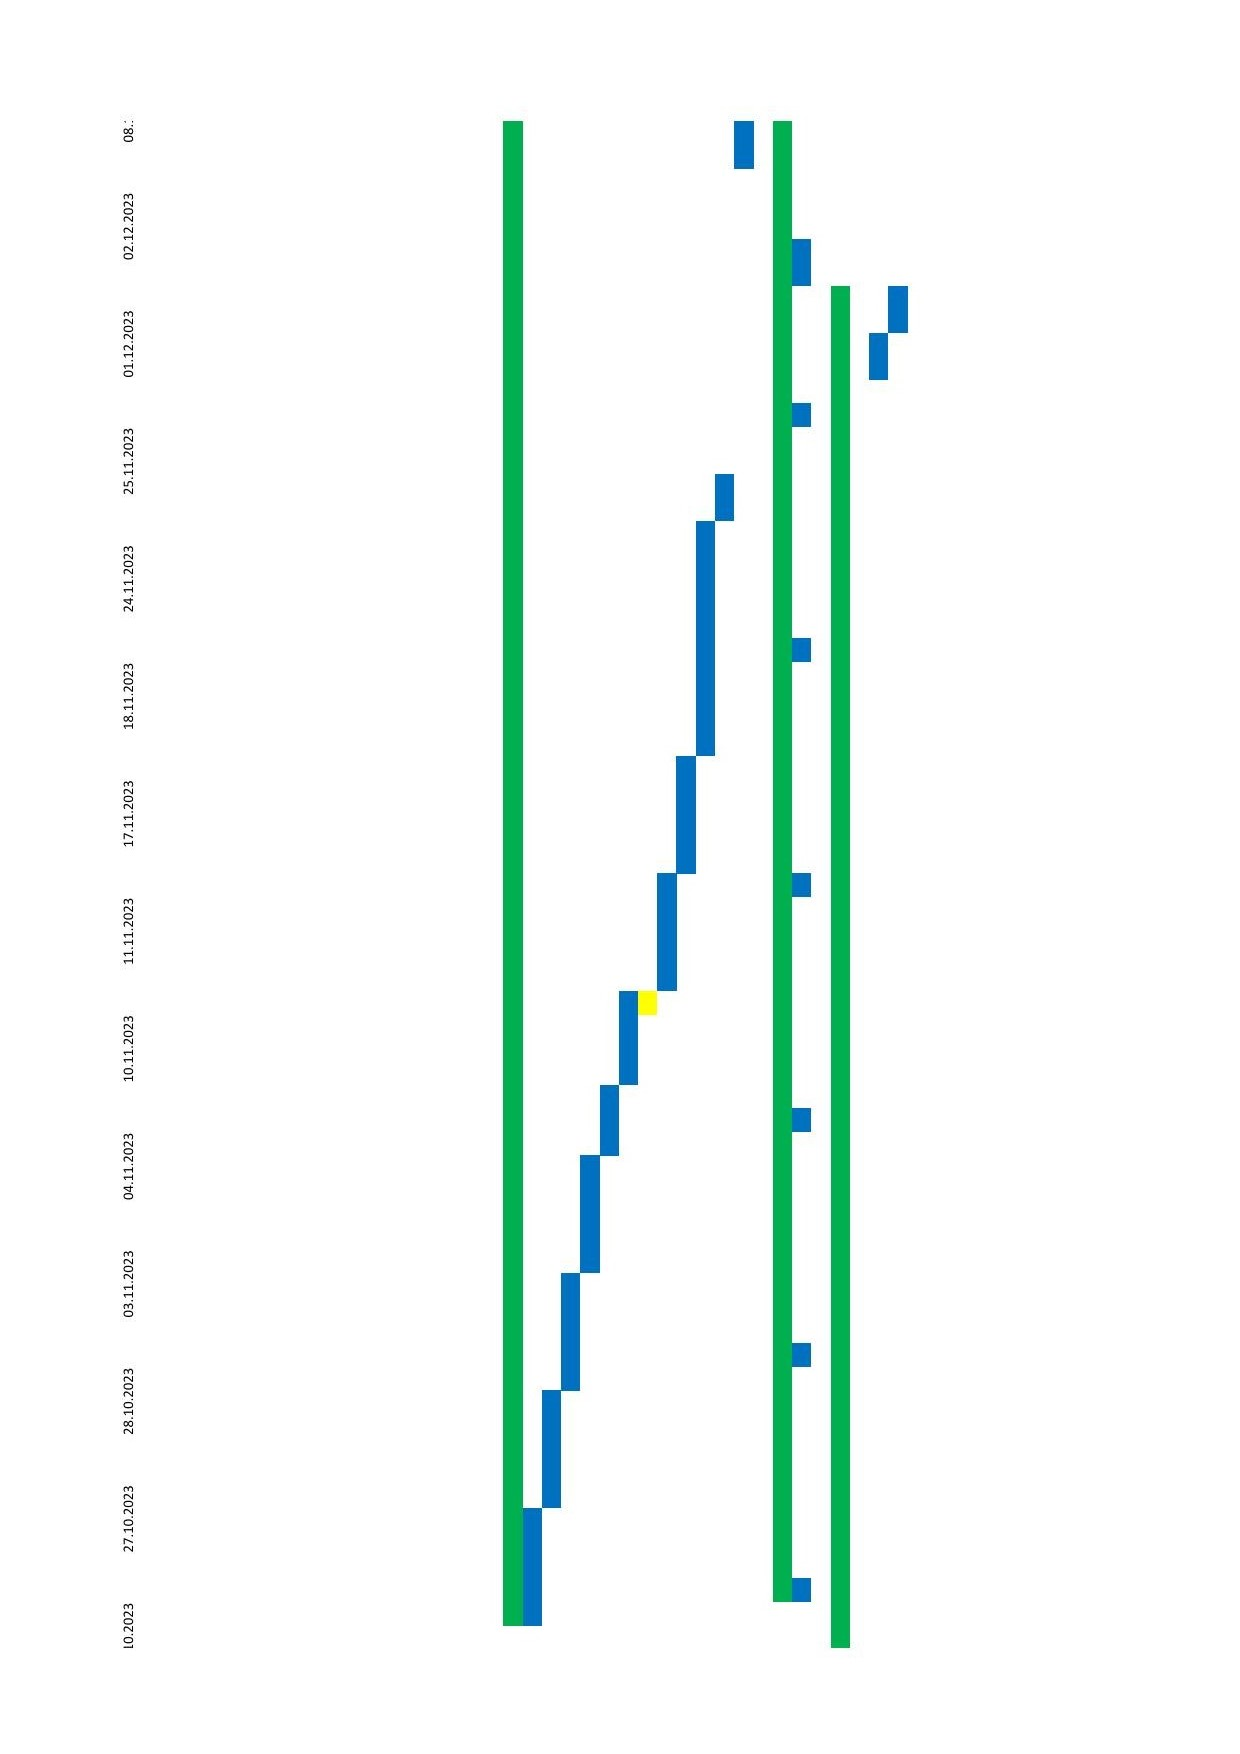
\includegraphics[width=\pdfpagewidth]{images/gantt2.jpg}
	\label{fig:planunggantt2}
\end{figure}

\begin{figure}[tb]
	\centering
		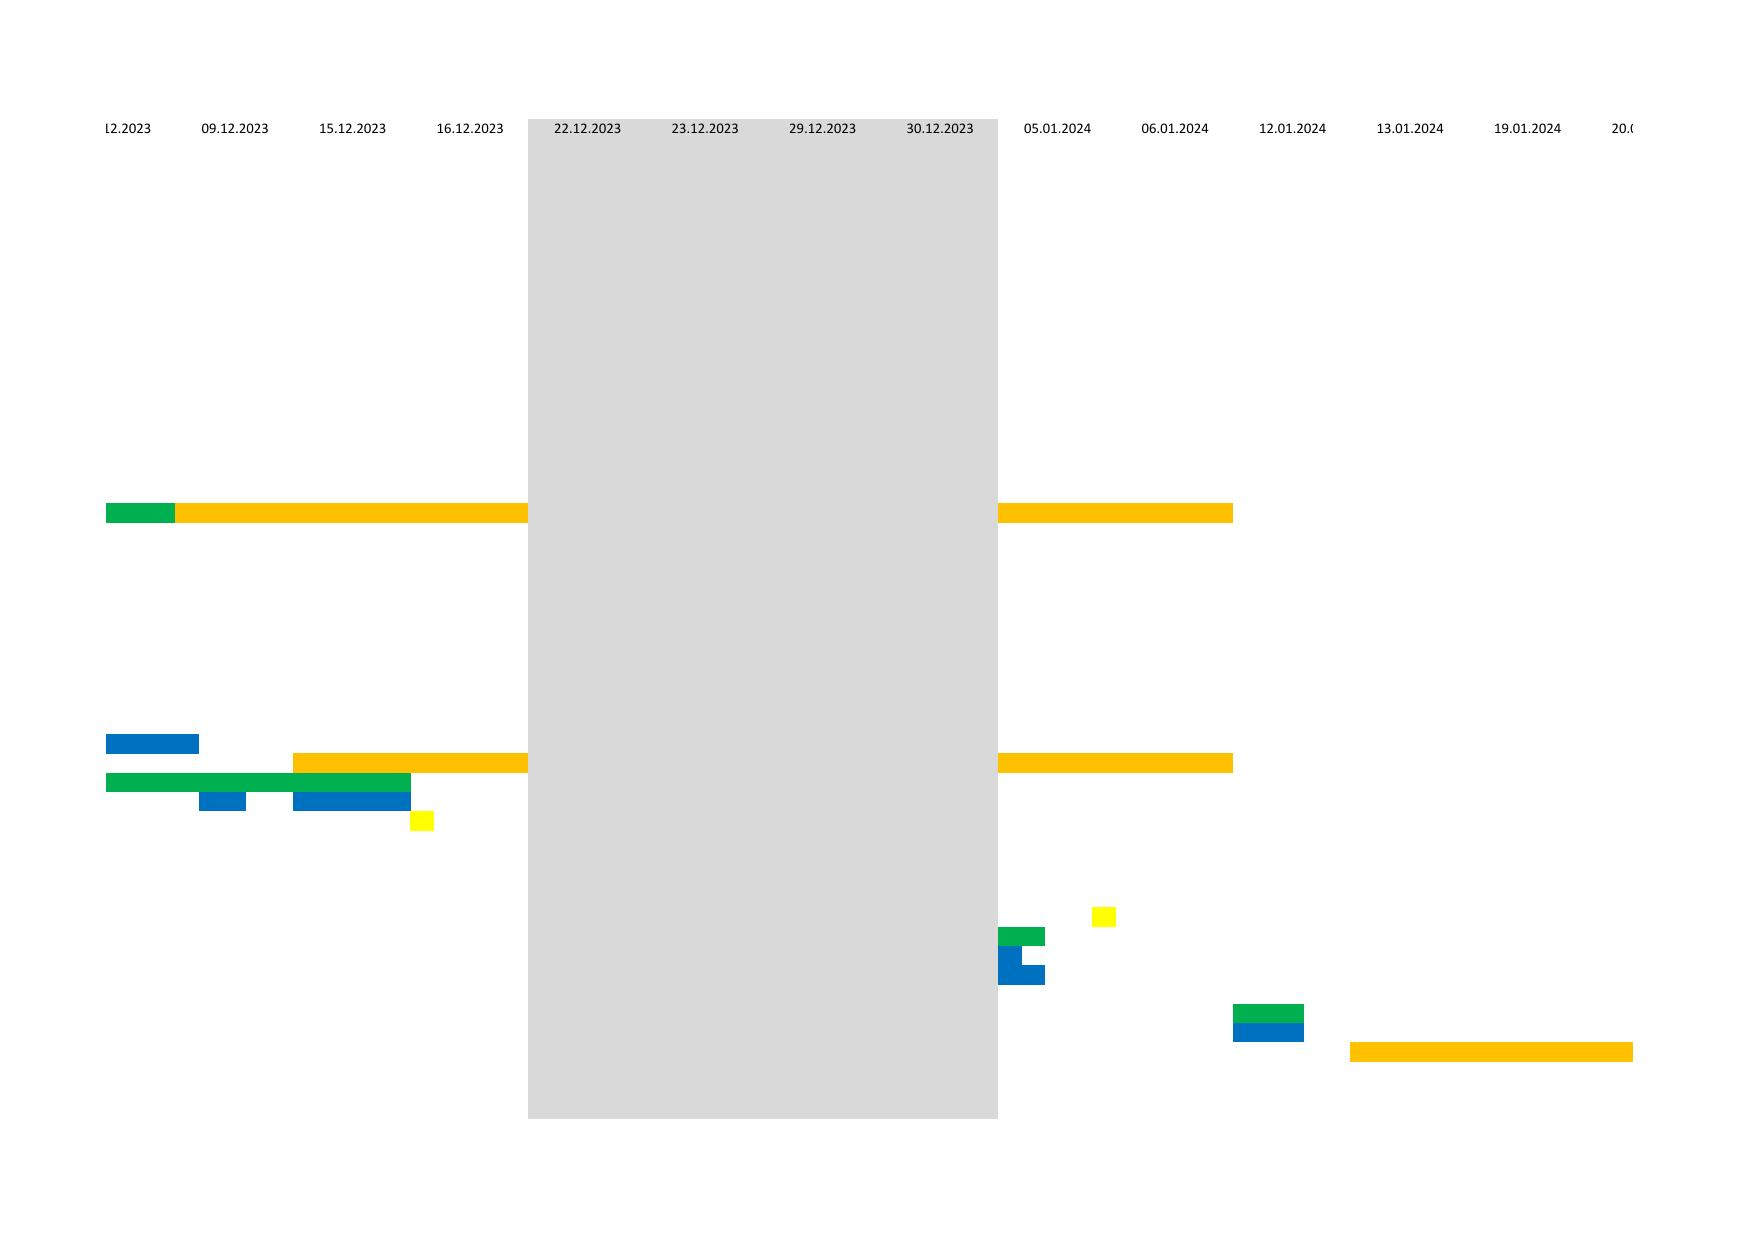
\includegraphics[width=\pdfpagewidth]{images/gantt3.jpg}
	\label{fig:planunggantt3}
\end{figure}

\begin{figure}[tb]
	\centering
		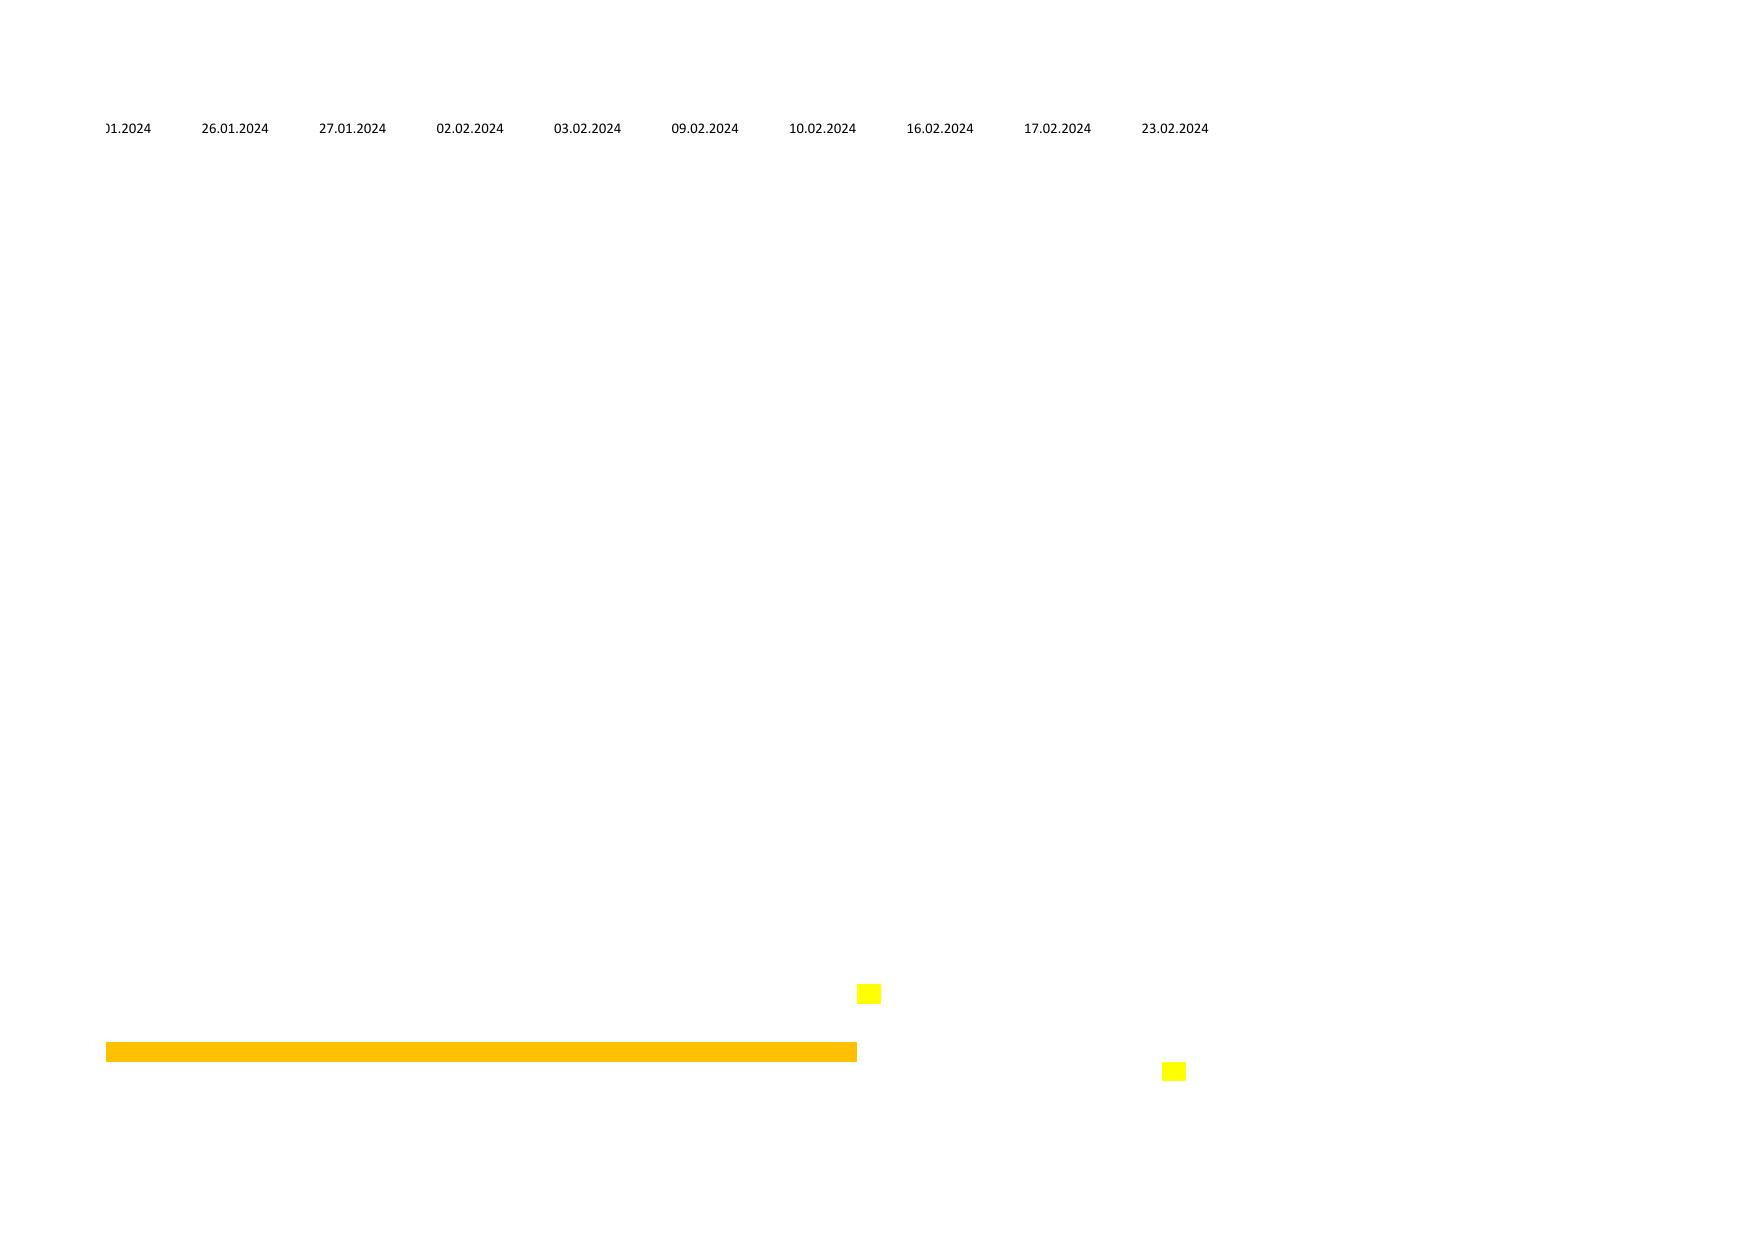
\includegraphics[width=\pdfpagewidth]{images/gantt4.jpg}
	\label{fig:planunggantt4}
\end{figure}
